% English version of the AQC paper
% Korean source: ../ko/main.tex
% Original draft: ../../AQC/main.tex
\documentclass[twocolumn,a4paper]{article}

\usepackage{../../AQC/nolta2025}
\usepackage{amsmath,amssymb,bbm,graphicx,subcaption,color,physics,hyperref,algorithm,algorithmic,txfonts}

\DeclareMathOperator*{\argmax}{arg\,max}
\DeclareMathOperator*{\argmin}{arg\,min}

\newcommand{\inp}[2]{\left\langle {#1} \middle| {#2} \right\rangle}
\newcommand{\kb}[1]{\ket{{#1}}\!\bra{{#1}}}
\newcommand{\bbE}{\mathbb{E}} \newcommand{\bbN}{\mathbb{N}} \newcommand{\bbB}{\mathbb{B}}
\newcommand{\bbS}{\mathbb{S}} \newcommand{\bbR}{\mathbb{R}} \newcommand{\bbC}{\mathbb{C}}
\newcommand{\bbZ}{\mathbb{Z}} \newcommand{\bbH}{\mathbb{H}} \newcommand{\bbQ}{\mathbb{Q}}
\newcommand{\calX}{\mathcal{X}} \newcommand{\calY}{\mathcal{Y}} \newcommand{\calZ}{\mathcal{Z}}
\newcommand{\calH}{\mathcal{H}} \newcommand{\calV}{\mathcal{V}} \newcommand{\BSC}{\mathrm{BSC}}

\newtheorem{theorem}{Theorem}
\newtheorem{corollary}[theorem]{Corollary}
\newtheorem{lemma}[theorem]{Lemma}
\newtheorem{proposition}[theorem]{Proposition}
\newtheorem{remark}{Remark}
\newtheorem{example}{Example}
\newtheorem{definition}{Definition}
\newtheorem{conjecture}{Conjecture}
\newtheorem{postulate}{Postulate}
\newtheorem{question}{Question}
\newtheorem{observation}{Observation}

\newenvironment{proof}{\par\noindent\textit{Proof.}\ }{\hfill\(\square\)\par\medskip}

\begin{document}

\title{Quantum Annealing-Based Optimization of
Pedestrian Network Orientation:
A QUBO Formulation Study for Preventing Crowd
Crush Disasters}
\author{YoHwan Lee${}^\dag$, Yunseong Jeong${}^\dag$, Se-Yeop Kim${}^\dag$, and Won-Joo Hwang${}^\ddag$}
\address{\dag School of Computer Science and Engineering, Pusan National University \\
\ddag Department of Information Convergence Engineering, Pusan National University \\
Busan 46241, Republic of Korea \\
Email: \email{dev.vackam@gmail.com}, \email{me@yunseong.dev}, \email{ksy1001k96@gmail.com}, \email{wjhwang@pusan.ac.kr}}
\maketitle
% \orcid{
% YoHwan Lee: TODO,
% Yunseong Jeong: TODO,
% Se-Yeop Kim: TODO,
% Won-Joo Hwang: 0000-0001-8398-564X
% }

\abstract
Crowd crush disasters can occur when dense pedestrian flows moving in opposite directions converge within narrow urban spaces, leading to a severe loss of individual mobility and control. To address this problem, this study proposes a quantum annealing-based orientation optimization framework for pedestrian networks. A pedestrian network is modeled as a weighted graph, where vertices represent intersections and edges represent walkable paths. The objective of the optimization is to assign traffic directions to paths in order to reduce conflicts between pedestrian flows, improve movement efficiency, and alleviate local congestion. To this end, the framework integrates three complementary strategies: a cycle-based approach, which preserves global circulation and network connectivity; an $n$-hop-based approach, which reduces overall travel distance; and a flow conservation approach, which balances inflow and outflow at each node. The final optimization problem is formulated as a Quadratic Unconstrained Binary Optimization (QUBO) model and solved on the D-Wave quantum annealing platform. Experimental results show that the proposed method reduces congestion, improves flow stability, and lowers the sum of all-pairs shortest paths (APSP), while requiring less computation time than conventional approaches.
\endabstract

\section{Introduction} \label{sec:intro}

Crowd crush disasters are a major public safety concern and have caused severe casualties in many settings~\cite{fruin1993causes}. These incidents arise not merely from high population density but from a complex interplay of factors, including environmental conditions such as topographical constraints and bottlenecks~\cite{helbing2007dynamics}, as well as insufficient initial responses to fallen individuals~\cite{soomaroo2012disasters}. The 2022 crowd disaster in South Korea further illustrates how extreme congestion in confined urban settings can rapidly become fatal~\cite{chang2024crowd}.

Various multifaceted solutions have been explored to prevent such crowd-related accidents~\cite{Nishinari2024}. However, real-world urban environments are immensely vast and complex, characterized by the simultaneous and real-time occurrence of unexpected variables such as road closures and bottlenecks. In these dynamically changing, large-scale environments, relying solely on classical computing resources presents clear limitations when attempting to account for all variables and derive optimal solutions in real time.

To overcome these challenges, this study abstracts the spatial characteristics of the target area into a graph. Building upon the foundational framework of quantum annealing~\cite{Kadowaki1998}, we directly formulate the crowd control optimization problem as a Quadratic Unconstrained Binary Optimization (QUBO) model. This formulation allows us to effectively leverage quantum hardware to rapidly derive optimal paths, thereby minimizing crowd density in large-scale congestion scenarios.

The contributions of our study are summarized as follows:
\begin{itemize}
    \setlength{\itemsep}{0pt}
    \setlength{\parsep}{0pt}
    \setlength{\parskip}{0pt}
    \item[(1)] Models the crowd control problem using a graph that captures complex urban networks and dynamic flows.
    \item[(2)] Proposes a novel QUBO formulation to efficiently solve large-scale routing problems via quantum annealing.
    \item[(3)] Demonstrates the viability of quantum computing for real-time disaster response through comparisons with classical algorithms.
\end{itemize}

The remainder of this paper is organized as follows. Section~\ref{sec:related} reviews related work. Section~\ref{sec:method} details the proposed method. Section~\ref{sec:result} presents the simulation results, and finally, Section~\ref{sec:conclusion} concludes this paper.

\section{Related Work} \label{sec:related}

\subsection{Crowd Safety and Pedestrian Flow Control} \label{subsec:related_crowd}

Previous studies on crowd safety have investigated pedestrian movement using microscopic crowd simulations, evacuation models, and flow-based approaches. These studies have shown that dense interactions among pedestrians can reduce walking speed, generate local bottlenecks, and increase the risk of unstable crowd movement. In transportation and evacuation planning, contraflow strategies have also been studied to improve the utilization of road capacity by reversing selected traffic directions during emergencies~\cite{kim2008contraflow, aksu2014mathematical}.

However, many existing approaches focus on operational crowd management or simulation-based analysis rather than the structural design of pedestrian circulation networks. In particular, relatively limited attention has been given to the optimization of one-way pedestrian path orientations as a preventive infrastructure-level measure.

\subsection{Graph-Based Network Orientation} \label{subsec:related_graph}

The problem of assigning directions to the edges of an undirected graph has been extensively studied in graph theory. Classical results have established conditions under which an undirected graph can be oriented while preserving strong connectivity~\cite{robbins1939theorem}. Subsequent studies have examined strongly connected orientations, network reliability, and optimal direction assignments in transportation networks~\cite{chung1985strongly, roberts1988optimal, roberts1994optimal}.

One-way street design has also been studied as a transportation network optimization problem. Existing approaches typically aim to reduce travel time, improve traffic capacity, or minimize the cost of modifying a road network~\cite{drezner1997selecting, huang2020bi, huang2020model}. Nevertheless, these problems become computationally challenging as the network size increases because the number of possible direction assignments grows exponentially with the number of edges. The complexity becomes even greater when strong connectivity, arc reversal, and multiple optimization objectives must be considered simultaneously~\cite{burkard1999minimum, bangjensen2023complexity}.

Unlike previous studies that primarily focus on vehicle transportation, this study considers pedestrian safety-oriented network orientation. The proposed formulation explicitly combines local flow balance, short-path reachability, and circulation preservation.

\subsection{Quantum Annealing for Combinatorial Optimization} \label{subsec:related_qa}

Quantum annealing has been applied to a variety of combinatorial optimization problems that can be expressed in Ising or QUBO form~\cite{qa_for_optimize}. Representative application domains include routing, scheduling, graph partitioning, and resource allocation. A QUBO model encodes binary decision variables and pairwise interactions into an energy function, allowing a quantum annealer to search for low-energy candidate solutions.

Practical execution on current quantum annealing hardware requires minor embedding, which maps logical variables and their interactions onto the limited connectivity of physical qubits~\cite{minor_embedding_inQA2, minor_embedding_inQA}. This embedding process may introduce additional overhead because a single logical variable can require a chain of multiple physical qubits. Therefore, the feasibility and quality of the embedding must be considered when designing a QA-compatible optimization model.

Building on these studies, we formulate the pedestrian network orientation problem as a QUBO model and evaluate its applicability on the D-Wave quantum annealing platform.

\section{System Model and Problem Formulation} \label{sec:model}

\subsection{Pedestrian Network and Decision Variables} \label{subsec:model_graph}

We consider an urban pedestrian environment represented by a weighted undirected graph $G=(V,E,W)$, where \(V\) denotes the set of pedestrian intersections, junctions, or decision points, and \(E\) denotes the set of walkable segments connecting them. Each undirected edge \(\{i,j\}\in E\) represents a physical pedestrian path that originally allows movement in both directions. A graph containing a bridge admits no strongly connected orientation at all~\cite{robbins1939theorem}. We therefore restrict the scope to ground-level pedestrian networks for which a planar, bridgeless approximation is valid, and assume that \(G\) is planar, connected, and bridgeless. Every block is then biconnected, so the face structure is well defined. In the experiments we use planar graphs generated by Delaunay triangulation.

The weight \(w_{ij}>0\) of each edge denotes its traversal capacity, which is proportional to the effective width and the walking capacity of the segment. The traversal cost of the segment, that is, its distance, is accordingly defined as the reciprocal
\begin{equation}
    \ell_{ij}=\frac{1}{w_{ij}}
\end{equation}
so that wider, higher-capacity paths are cheaper to traverse. Because counter-flow along narrow paths degrades walking efficiency, the objective of this study is to transform the original bidirectional pedestrian network into a directed one-way circulation network by assigning a single walking direction to each pedestrian segment.

For each undirected edge \(\{i,j\}\in E\), an arbitrary but fixed ordering of its endpoints is imposed such that \(i<j\), and a binary orientation variable \(x_{ij}\) is defined so that \(x_{ij}=0\) orients the edge as \(i\rightarrow j\) and \(x_{ij}=1\) orients it as \(j\rightarrow i\). The complete variable vector \(\mathbf{X}\in\{0,1\}^{|E|}\) fully determines the directed graph \(\vec{G}(\mathbf{X})=(V,\vec{E}(\mathbf{X}))\), and each physical pedestrian segment is assigned exactly one direction. For notational brevity the definitions below index variables by endpoint pairs, but series contraction (Section~\ref{subsec:method_pre}) can create more than one edge joining the same pair of endpoints. In that case variables and indicator functions are distinguished by edge identifier, and every sum over \(\mathrm{adj}(v)\) is read as a sum over the edges incident to \(v\).

To simplify the exposition, we first define a direction indicator function for an ordered pair \((a,b)\) of adjacent nodes. For \(\{a,b\}\in E\), we set \(\rho_{ab}(\mathbf{X})=1-x_{ab}\) if \(a<b\), and \(\rho_{ab}(\mathbf{X})=x_{ba}\) if \(b<a\). The quantity \(\rho_{ab}\) is not an additional decision variable but a compact expression determined entirely by \(\mathbf{X}\); it equals one when the arc \(a\rightarrow b\) exists in \(\vec{G}(\mathbf{X})\), and it always satisfies \(\rho_{ab}+\rho_{ba}=1\). The set of vertices adjacent to \(v\) is denoted by \(\mathrm{adj}(v)\).

\subsection{Movement Efficiency Objective}

Orientation inevitably forces some trips onto detours, so the degree to which the directed network still supports efficient movement becomes the target of the optimization. Let \(D_{st}(\mathbf{X})\) denote the shortest directed-path distance from a source node \(s\) to a destination node \(t\) in \(\vec{G}(\mathbf{X})\), computed with respect to the edge distances \(\ell_{ij}=1/w_{ij}\), and let \(\bar{D}_{st}\) denote the corresponding shortest distance in the undirected graph \(G\) before orientation. If no directed path from \(s\) to \(t\) exists, we set \(D_{st}(\mathbf{X})=\infty\).

How much orientation inflates distances is a long-standing question in graph theory~\cite{chvatal1978distances}. Rather than measuring movement efficiency as an absolute sum of distances, we measure it as the detour ratio induced by orientation. The normalized all-pairs shortest-path cost is defined as
\begin{equation}
F_{\mathrm{dist}}(\mathbf{X})=\frac{1}{|V|(|V|-1)}\sum_{\substack{s,t\in V\\s\neq t}}\frac{D_{st}(\mathbf{X})}{\bar{D}_{st}}
\label{eq:stretch}
\end{equation}
Since \(D_{st}\geq\bar{D}_{st}\) always holds, we have \(F_{\mathrm{dist}}(\mathbf{X})\geq1\), and values closer to one indicate that the orientation preserves the original walking distances more faithfully. This metric is invariant to graph size and weight scale, so networks of different sizes can be compared. The experiments in Section~\ref{sec:result}, however, recorded the unnormalized mean directed distance \(D_{\mathrm{avg}}(\mathbf{X})=\frac{1}{|V|(|V|-1)}\sum_{s\neq t}D_{st}(\mathbf{X})\), which therefore cannot be used for cross-size comparison. Cross-size comparison is instead carried out in Section~\ref{sec:result} with an approximation obtained by dividing by the undirected reference distance (Figure~\ref{fig:stretch}).

For \eqref{eq:stretch} to be meaningful, \(\vec{G}(\mathbf{X})\) must be strongly connected. We denote by \(\mathcal{X}_{\mathrm{sc}}\) the set of all \(\mathbf{X}\) for which \(\vec{G}(\mathbf{X})\) is strongly connected.

\subsection{Short-Path Reachability Surrogate} \label{subsec:model_hop}

The objective \(F_{\mathrm{dist}}\) in \eqref{eq:stretch} is a nonlocal function that depends on the global orientation pattern of the entire graph, and it therefore cannot be written directly as a quadratic form. We accordingly introduce a local reachability surrogate that encourages the formation of short directed paths. Using \(\rho\), the weighted count of all directed walks \((v_0,v_1,\dots,v_n)\) of length \(n\) consisting of distinct vertices can be written as
\begin{equation}
P_n(\mathbf{X})=\sum_{(v_0,\dots,v_n)}\;\prod_{r=1}^{n}w_{v_{r-1}v_r}\,\rho_{v_{r-1}v_r}(\mathbf{X})
\label{eq:pn}
\end{equation}
where the sum ranges over all walks with \(v_r\neq v_{r'}\ (r\neq r')\) and \(\{v_{r-1},v_r\}\in E\ (1\leq r\leq n)\). In the presence of parallel edges the terms are distinguished by the edge sequence, but the distinctness requirement still applies to vertices.

Although \(P_n\) is formally of degree \(n\), walks pair with their reversals and the leading-degree terms may cancel.

\begin{proposition} \label{prop:deg}
Let \(n\geq1\), and allow some edges to have a constant, fixed orientation (the pre-oriented boundary edges of Section~\ref{subsec:method_pre}). Then \(P_n\) is a polynomial of degree at most \(n-1\) when \(n\) is odd, and of degree at most \(n\) when \(n\) is even. In particular, both \(P_2\) and \(P_3\) are of degree at most two.
\end{proposition}

\begin{proof}
The sum in \eqref{eq:pn} is closed under reversal of walks, and since the vertices are distinct we have \(v_0\neq v_n\), so reversal is a fixed-point-free involution. The weight products of a reversal pair coincide by the symmetry of \(w\). If every edge traversed by the pair is free, then writing \(\rho_r=\rho_{v_{r-1}v_r}\), the reversed walk contributes the factor \(1-\rho_r\), so the pair sums to \(\prod_rw_r\bigl[\prod_r\rho_r+\prod_r(1-\rho_r)\bigr]\). Because the vertices are distinct, the \(n\) edges are pairwise distinct and each \(\rho_r\) equals either \(x_{e_r}\) or \(1-x_{e_r}\). Letting \(k\) be the number of indices \(r\) with \(\rho_r=1-x_{e_r}\), the coefficient of \(\prod_rx_{e_r}\) is \((-1)^k\) in the first term and \((-1)^{n-k}\) in the second, summing to \((-1)^k\bigl(1+(-1)^n\bigr)\). The leading term therefore cancels for odd \(n\) and doubles for even \(n\). If at least one edge traversed by the pair is pre-oriented, its factor is a constant and the walk that disagrees with that orientation vanishes because its factor is zero; the surviving term then involves at most \(n-1\) variables, so the pair already contributes degree at most \(n-1\) regardless of parity.
\end{proof}

The bound of Proposition~\ref{prop:deg} is \(n-1\) for odd \(n\) and \(n\) for even \(n\), so the only hop lengths guaranteed to yield a quadratic form are \(n\in\{2,3\}\). This is one further reason for restricting the hop length to these two values. The quantity \(P_n\) measures the extent to which an orientation supports short-range and intermediate-range reachability, and maximizing it serves as a structural proxy for reducing unnecessary detours. We therefore define the short-path reachability objective as
\begin{equation}
F_{\mathrm{hop}}(\mathbf{X})=-\lambda_2P_2(\mathbf{X})-\lambda_3P_3(\mathbf{X})
\end{equation}

\subsection{Problem Formulation}

Combining the above, the pedestrian network orientation problem is formulated as a binary constrained optimization problem. The only decision variable is the binary orientation vector \(\mathbf{X}\), and with the exact objective the problem reads
\begin{equation}
\min_{\mathbf{X}\in\mathcal{X}_{\mathrm{sc}}}\quad F_{\mathrm{dist}}(\mathbf{X})
\label{eq:exact}
\end{equation}
Problem~\eqref{eq:exact} cannot be submitted to a quantum annealer directly, because \(F_{\mathrm{dist}}\) is nonlocal and \(\mathcal{X}_{\mathrm{sc}}\) is a nonconvex combinatorial constraint. The distance criterion is evaluated only during sample selection and final assessment, and the ranking is performed with the unnormalized distance \(D_{\mathrm{avg}}\), which differs from \(F_{\mathrm{dist}}\) only in the per-pair weighting.

\section{Proposed Method} \label{sec:method}

\subsection{Framework Overview}

The proposed framework consists of two components. Preprocessing (series contraction and face partitioning) first establishes a circulation skeleton linking the clusters, which lowers the global strong-connectivity requirement to the local condition that each subgraph be strongly connected (Proposition~\ref{prop:sc}); the energy function then retains only the reachability term that maximizes short directed paths. Strong connectivity is not a deterministic guarantee but the conditional conclusion of Proposition~\ref{prop:sc}.

There are two reasons for not imposing strong connectivity as a penalty term. First, strong connectivity is not a local condition, so it admits no low-degree polynomial representation, and forcing one causes an explosion of auxiliary variables. Second, although a sufficiently large penalty makes the global optimum feasible, its large energy scale erodes the effective resolution of the annealer and makes fine differences between objective terms indistinguishable. Establishing the circulation skeleton during preprocessing avoids both problems as far as the strong-connectivity constraint is concerned, and the pre-oriented edges become constants, which additionally reduces the number of logical variables.

\subsection{Preprocessing: Series Contraction and Face Partitioning} \label{subsec:method_pre}

\subsubsection*{Series Contraction}

In a path-shaped chain of degree-two vertices \(a-u_1-\cdots-u_k-b\), each internal vertex has exactly two incident edges. If even a single edge inside the chain is oriented against the rest, some \(u_r\) has in-degree or out-degree zero and strong connectivity is destroyed. In any strongly connected solution the entire chain is therefore bound to a single binary decision. This means that series contraction, which removes degree-two vertices and replaces the chain by one equivalent edge, preserves the feasible set while reducing \(k+1\) variables to one.

The capacity of the equivalent edge is determined by the series composition law. Since the traversal cost \(\ell=1/w\) is additive along the chain, we have \(\ell_{\mathrm{eq}}=\sum_{r=1}^{k+1}\ell_r\) and therefore
\begin{equation}
    w_{\mathrm{eq}}=\Bigl(\textstyle\sum_{r}1/w_{r}\Bigr)^{-1}
\end{equation}
This composition makes the shortest distances of the contracted graph exactly equal to those of the original.

A chain whose two endpoints coincide already forms a cycle and thus does not affect strong connectivity; such pendant cycles are removed during contraction and excluded from the decision variables, then reinjected with a fixed orientation during restoration. This choice affects \(D_{st}\) only for pairs involving vertices inside that cycle. Because the removal lowers the degree of adjacent vertices and can create new contraction candidates, the procedure is repeated until no contractible chain remains.

\subsubsection*{Face Partitioning and Boundary Orientation}

For each biconnected component of the contracted graph, we enumerate the planar faces and identify the face of maximum area as the outer face, which is excluded (a heuristic). Clustering the remaining internal faces by $k$-means over their centroid coordinates makes every edge shared by two faces in different clusters a cluster boundary. An outer edge, which is incident to only one internal face, always belongs to the boundary, so the entire outer perimeter of the network becomes subject to pre-orientation.

For the boundary to decompose into cycles, every vertex must have even boundary degree. If vertices of odd degree remain, we compute a minimum-weight perfect matching among them and add to the boundary the symmetric difference of the shortest paths joining the matched vertices. This symmetric difference is a minimum-cost \(T\)-join for the set of odd vertices, so after correction every vertex has even degree; together with the matching it is computed in polynomial time~\cite{edmonds1973matching}. Outer edges are assigned a sufficiently large finite cost so that the correction paths do not cut the outer perimeter.

Since each cycle of the corrected boundary is a closed curve in the plane, coloring the faces by the parity of the number of cycles enclosing them makes exactly the two faces separated by a boundary edge differ in color. The merged dual graph, whose vertices are the clusters and whose edges are the shared boundaries, is therefore always bipartite and admits a 2-coloring. Assigning opposite traversal orientations to adjacent clusters according to this coloring, and fixing the direction of each boundary edge from the traversal order of the incident face, makes the two prescriptions agree on shared boundaries and turns the boundary into directed cycles in which in-degree equals out-degree at every vertex.

Each subgraph then consists of the undirected internal edges of one cluster (the decision variables) together with its boundary edges (already oriented constants). Face components that leak to the outer face are excluded from the clusters, and both the excluded components and any residual edges assigned to no cluster are left unoriented.

\subsection{QUBO Formulation} \label{subsec:method_qubo}

For each subgraph we use the surrogate objective of Section~\ref{subsec:model_hop} directly as the energy function:
\begin{equation}
    H(\mathbf{X})=F_{\mathrm{hop}}(\mathbf{X})=-\lambda_2P_2(\mathbf{X})-\lambda_3P_3(\mathbf{X})
\label{eq:hamiltonian}
\end{equation}
By Proposition~\ref{prop:deg}, \(P_2\) and \(P_3\) are of degree at most two, so \(H\) is already a QUBO without auxiliary variables, and the logical variables correspond one-to-one to the undirected edges. The absence of a strong-connectivity penalty term is the distinguishing feature of this formulation; the boundary cycles of Section~\ref{subsec:method_pre} and Proposition~\ref{prop:sc} take its place. Pre-oriented boundary edges enter as constants. The experiments use \(\lambda_2=\lambda_3=1\).

\begin{remark} \label{rmk:flow}
The energy function of the implementation used in the experiments additionally includes the sum of squared differences between the outgoing and incoming capacities at each vertex (a flow-balance term). In a simple graph, however, \(\rho_{uv}\rho_{vu}=0\), so grouping this term by its middle vertex makes it equal to a constant minus \(4P_2\); adding the term is therefore exactly equivalent to raising \(\lambda_2\) from 1 to 5. No contraction was applied to the experimental instances, so there are no parallel edges and the equivalence is exact. The experimental results should thus be read as results for \eqref{eq:hamiltonian} with \(\lambda_2=5\) and \(\lambda_3=1\).
\end{remark}

\subsection{Problem Size} \label{subsec:method_partition}

Since there are no auxiliary variables, the number of logical variables of subgraph \(p\) equals its number of internal edges \(m_p\), which series contraction and boundary pre-orientation jointly reduce. What determines the size submitted to the annealer, however, is the number of couplings rather than the number of variables. Whereas \(P_2\) connects only edge pairs sharing a vertex, \(P_3\) also connects edge pairs at distance two, so the coupling count grows on the order of \(\sum_{\{u,v\}\in E}\deg(u)\deg(v)\); for planar graphs of average degree around five this is roughly \(17m_p\) (measured in Section~\ref{sec:result}). The coupler budget therefore saturates before the qubit budget.

Because embeddability limits the subgraph size, the target cluster count \(k\) directly controls this scale. A small \(k\) yields large subgraphs that are hard to embed, whereas a large \(k\) pre-orients more boundary edges and reduces the degrees of freedom of the solution. We therefore choose \(k\) as small as possible subject to every subgraph passing the embedding test; the implementation locates it by binary search over \(k\), so minimality is guaranteed only when the pass/fail outcome is monotone in \(k\). The test applies two cheap prescreens (comparing the number of undirected edges and the number of variables against the vertex count of the target topology) and then runs an actual minor-embedding search, passing if an embedding is found. This search is heuristic, so it may reject an embeddable subgraph, and above all the cost of a failure verdict is high enough to dominate the runtime of the whole pipeline. Embeddings that are found are reused as fixed embeddings during sampling. Placing a stronger prescreen, such as the degeneracy of the interaction graph, in front of the search is a natural improvement but was not included in this experimental configuration. Note also that \(k\) is only a target: the actual number of subgraphs is determined by the number of connected components of faces, after boundary correction, that do not leak to the outer face.

\subsection{Merging and Restoration}

When selecting a solution from the samples of each subgraph, we do not take the lowest-energy sample. Because \eqref{eq:hamiltonian} is a surrogate objective, minimum energy does not imply a minimum of \(F_{\mathrm{dist}}\). Instead, each sample is restored to a directed graph and ranked by the sum of directed shortest-path distances. A sample that is not strongly connected has \(F_{\mathrm{dist}}=\infty\), so whenever at least one strongly connected sample exists it is the one selected.

The partial solutions are merged edge by edge, fixed on the original graph, and the full graph is then solved once more. Edges that are already fixed enter both objective terms as constants, so the decision variables of this final solve are restricted to the residual edges. Finally, the orientation of each equivalent edge is propagated to the edges of its original chain and the removed pendant cycles are reinjected, restoring the solution \(\mathbf{X}^{*}\) on the original graph. Evaluation is performed on the original graph, not on the contracted one.

The conditions under which global strong connectivity follows are summarized below.

\begin{proposition} \label{prop:sc}
By the assumptions of Section~\ref{subsec:model_graph}, \(G\) is connected and bridgeless, and series contraction preserves both properties. Assume the following for every biconnected component of the contracted graph. (i) The merged dual graph of that component is connected. (ii) The directed subgraph \(\vec{G}_p\) of each subgraph \(p\) is strongly connected. (iii) Every vertex of the component belongs to at least one of the subgraphs generated from it, and merging preserves the orientations of the partial solutions. Then the restored directed graph \(\vec{G}(\mathbf{X}^{*})\) is strongly connected.
\end{proposition}

\begin{proof}
Two adjacent clusters share a boundary edge, so the corresponding subgraphs share a vertex, and the union of two strongly connected directed graphs sharing a vertex is strongly connected. By assumption (i) any two subgraphs are joined by a sequence of adjacent subgraphs, so \(\bigcup_p\vec{G}_p\) is strongly connected by induction; by assumption (iii) this union is a spanning subgraph, hence the orientation of the component is strongly connected regardless of how the residual edges are oriented. The restoration step expands the orientation of an equivalent edge uniformly along the whole chain and reinjects pendant cycles as directed cycles, so it preserves reachability. If there are several components, the same argument is applied to the block-cut tree.
\end{proof}

The proposed construction does not deterministically produce a strongly connected orientation. Assumption (ii) holds only when the sample set returned by the annealer contains a strongly connected sample, and assumption (iii) fails whenever a component is excluded due to outer leakage. The role of this construction is therefore to lower a global condition to the subgraph level and thereby raise its attainability; whether it is actually attained is confirmed by the strong-connectivity rate reported in Section~\ref{sec:result}.

\section{Simulation Results} \label{sec:result}

\subsection{Experimental Setup}

The targets are Delaunay-triangulated planar graphs with \(|V|\in\{100,200,300,400,500\}\) vertices, with three instances generated per size and averages reported. All edge weights are set to \(w_{ij}=1\), so \(\ell_{ij}=1\). The QUBO is constructed without normalization using \(\lambda_2=\lambda_3=1\), and the flow-balance term of Remark~\ref{rmk:flow} is included with weight one, giving an effective \(\lambda_2\) of 5.

We compare the proposed method against four classical methods. The proposed method applies the partitioning of Section~\ref{sec:method} and samples each subgraph QUBO on a D-Wave quantum annealer (\texttt{num\_reads}=100 per subgraph, chain strength left at the sampler default policy, and the embedding found during partitioning reused through a fixed-embedding composite). \emph{Raw SA} is simulated annealing that searches orientations directly, \emph{ILS} is iterated local search, \emph{Robbins} is the classical method that constructs a strongly connected orientation by depth-first search~\cite{robbins1939theorem}, and \emph{Random} is a random orientation. The embedding search uses minorminer~\cite{cai2014practical} with default settings (a search budget of 1{,}000 seconds), and the target topology is the working-qubit graph of the actual QPU. The embeddability of the unpartitioned whole-graph QUBO is measured separately against an ideal Pegasus \(P_{16}\) topology (5{,}640 qubits) in Section~\ref{subsec:result_embed}.

\subsection{Problem Size and Embeddability} \label{subsec:result_embed}

Figure~\ref{fig:scalability} shows the number of BQM binary variables. Without partitioning the variable count grows in proportion to \(|V|\), reaching 1{,}481; with partitioning the largest subgraph averages between 263 and 365 variables (the maximum over individual instances is 428). Even the total, at 1{,}346, is smaller than the unpartitioned count, because pre-oriented boundary edges are removed from the variable set.

\begin{figure}[t]
\centering
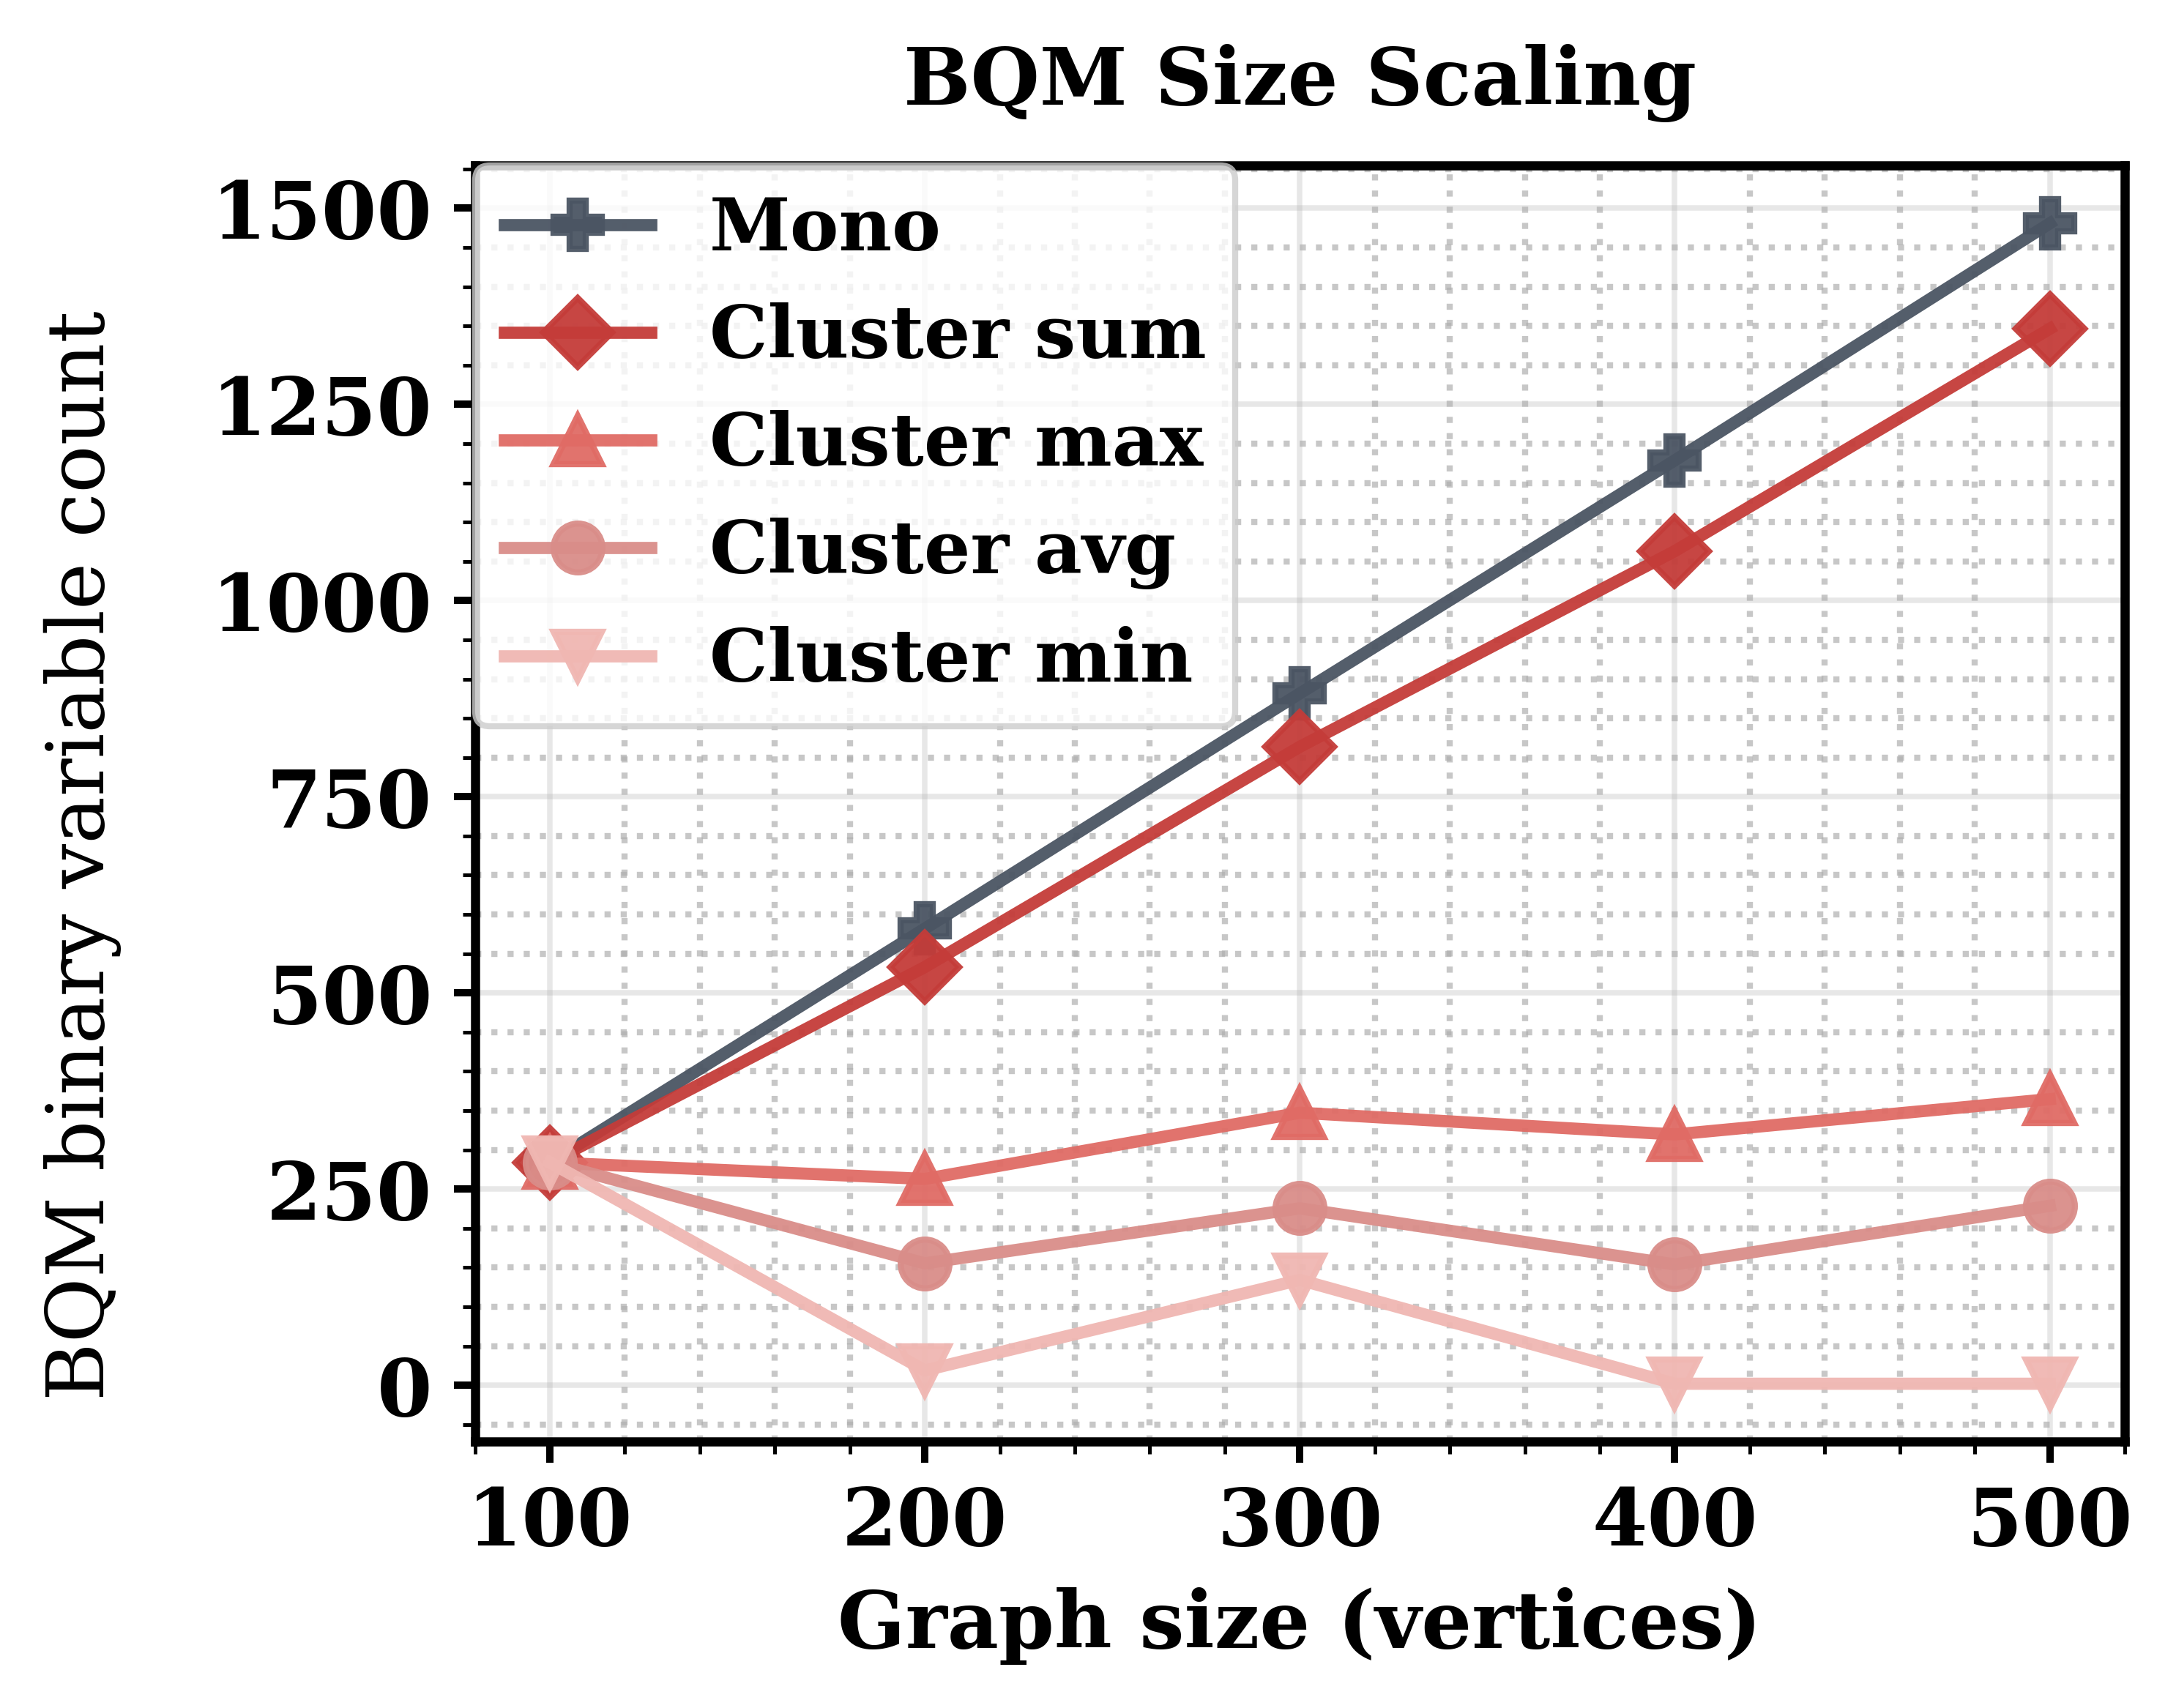
\includegraphics[width=\linewidth]{../ko/fig/scalability.png}
\caption{Number of BQM binary variables. Mono denotes the unpartitioned whole-graph QUBO, while Cluster sum/max/avg/min denote the total, maximum, average, and minimum over the subgraphs produced by the proposed partitioning.}
\label{fig:scalability}
\end{figure}

This difference decides embeddability. Without partitioning, the \(|V|=100\) case embeds into 3{,}008 physical qubits on average, but for \(|V|\geq200\) no embedding is found within the default search budget of 1{,}000 seconds (search times of 1{,}021--1{,}064 seconds all sit at the budget). This is not a proof of non-embeddability but a failure of a heuristic search; a larger budget or a different embedding algorithm could change the outcome. With partitioning, by contrast, every subgraph embeds up to \(|V|=500\), and the largest number of physical qubits used by a single subgraph is 4{,}391 (\(|V|=300\), 405 logical variables), within the 5{,}640 available. That 582 logical variables fail to embed into the ideal topology while 428 embed into 4{,}181 physical qubits on the harsher real working graph is consistent in direction with the coupler-first saturation predicted in Section~\ref{subsec:method_partition}. This appears to be because the \(P_3\) term also connects edge pairs at distance two, so the coupling density grows faster than the variable count; this experiment did not record per-subgraph coupling counts, however, so the asymmetry was not verified directly (whole-graph coupling measurements appear in Section~\ref{subsec:result_ablation}).

\subsection{Solution Quality}

Figure~\ref{fig:apsp} reports \(D_{\mathrm{avg}}\) by method. Strongly connected orientations were obtained by ILS and Robbins in all 15 trials, by the proposed method in all 14 completed trials (one \(|V|=200\) trial aborted during partitioning), and by Raw SA only in the 9 trials with \(|V|\leq300\). Robbins guarantees strong connectivity but yields \(D_{\mathrm{avg}}=65.8\) at \(|V|=500\), more than six times that of the proposed method. For Random, not a single one of the random samples (30 per size, 150 in total) was strongly connected, so \(D_{\mathrm{avg}}\) is undefined. Raw SA attains a lower \(D_{\mathrm{avg}}\) for \(|V|\leq300\) but fails to obtain a strongly connected orientation for \(|V|\geq400\). This advantage must, however, be read together with the computational cost. Over the \(|V|\leq300\) range where the advantage holds, the per-instance search time of Raw SA is 4.7--11.8 times the total time of the proposed method (partitioning and embedding search plus QUBO solving), namely 24{,}936 seconds against 2{,}584 seconds at \(|V|=300\). At \(|V|=500\), where Raw SA obtains no strongly connected orientation, the gap widens to roughly 24 times: 101{,}597 seconds against 4{,}260 seconds. \emph{ILS} attains the lowest \(D_{\mathrm{avg}}\) at every size, which is because ILS minimizes the evaluation metric directly whereas the QUBO-based methods minimize the surrogate objective \(H\). The per-instance time of ILS at \(|V|=500\) is 44{,}862 seconds, 10.5 times the total time of the proposed method.

\begin{figure}[t]
\centering
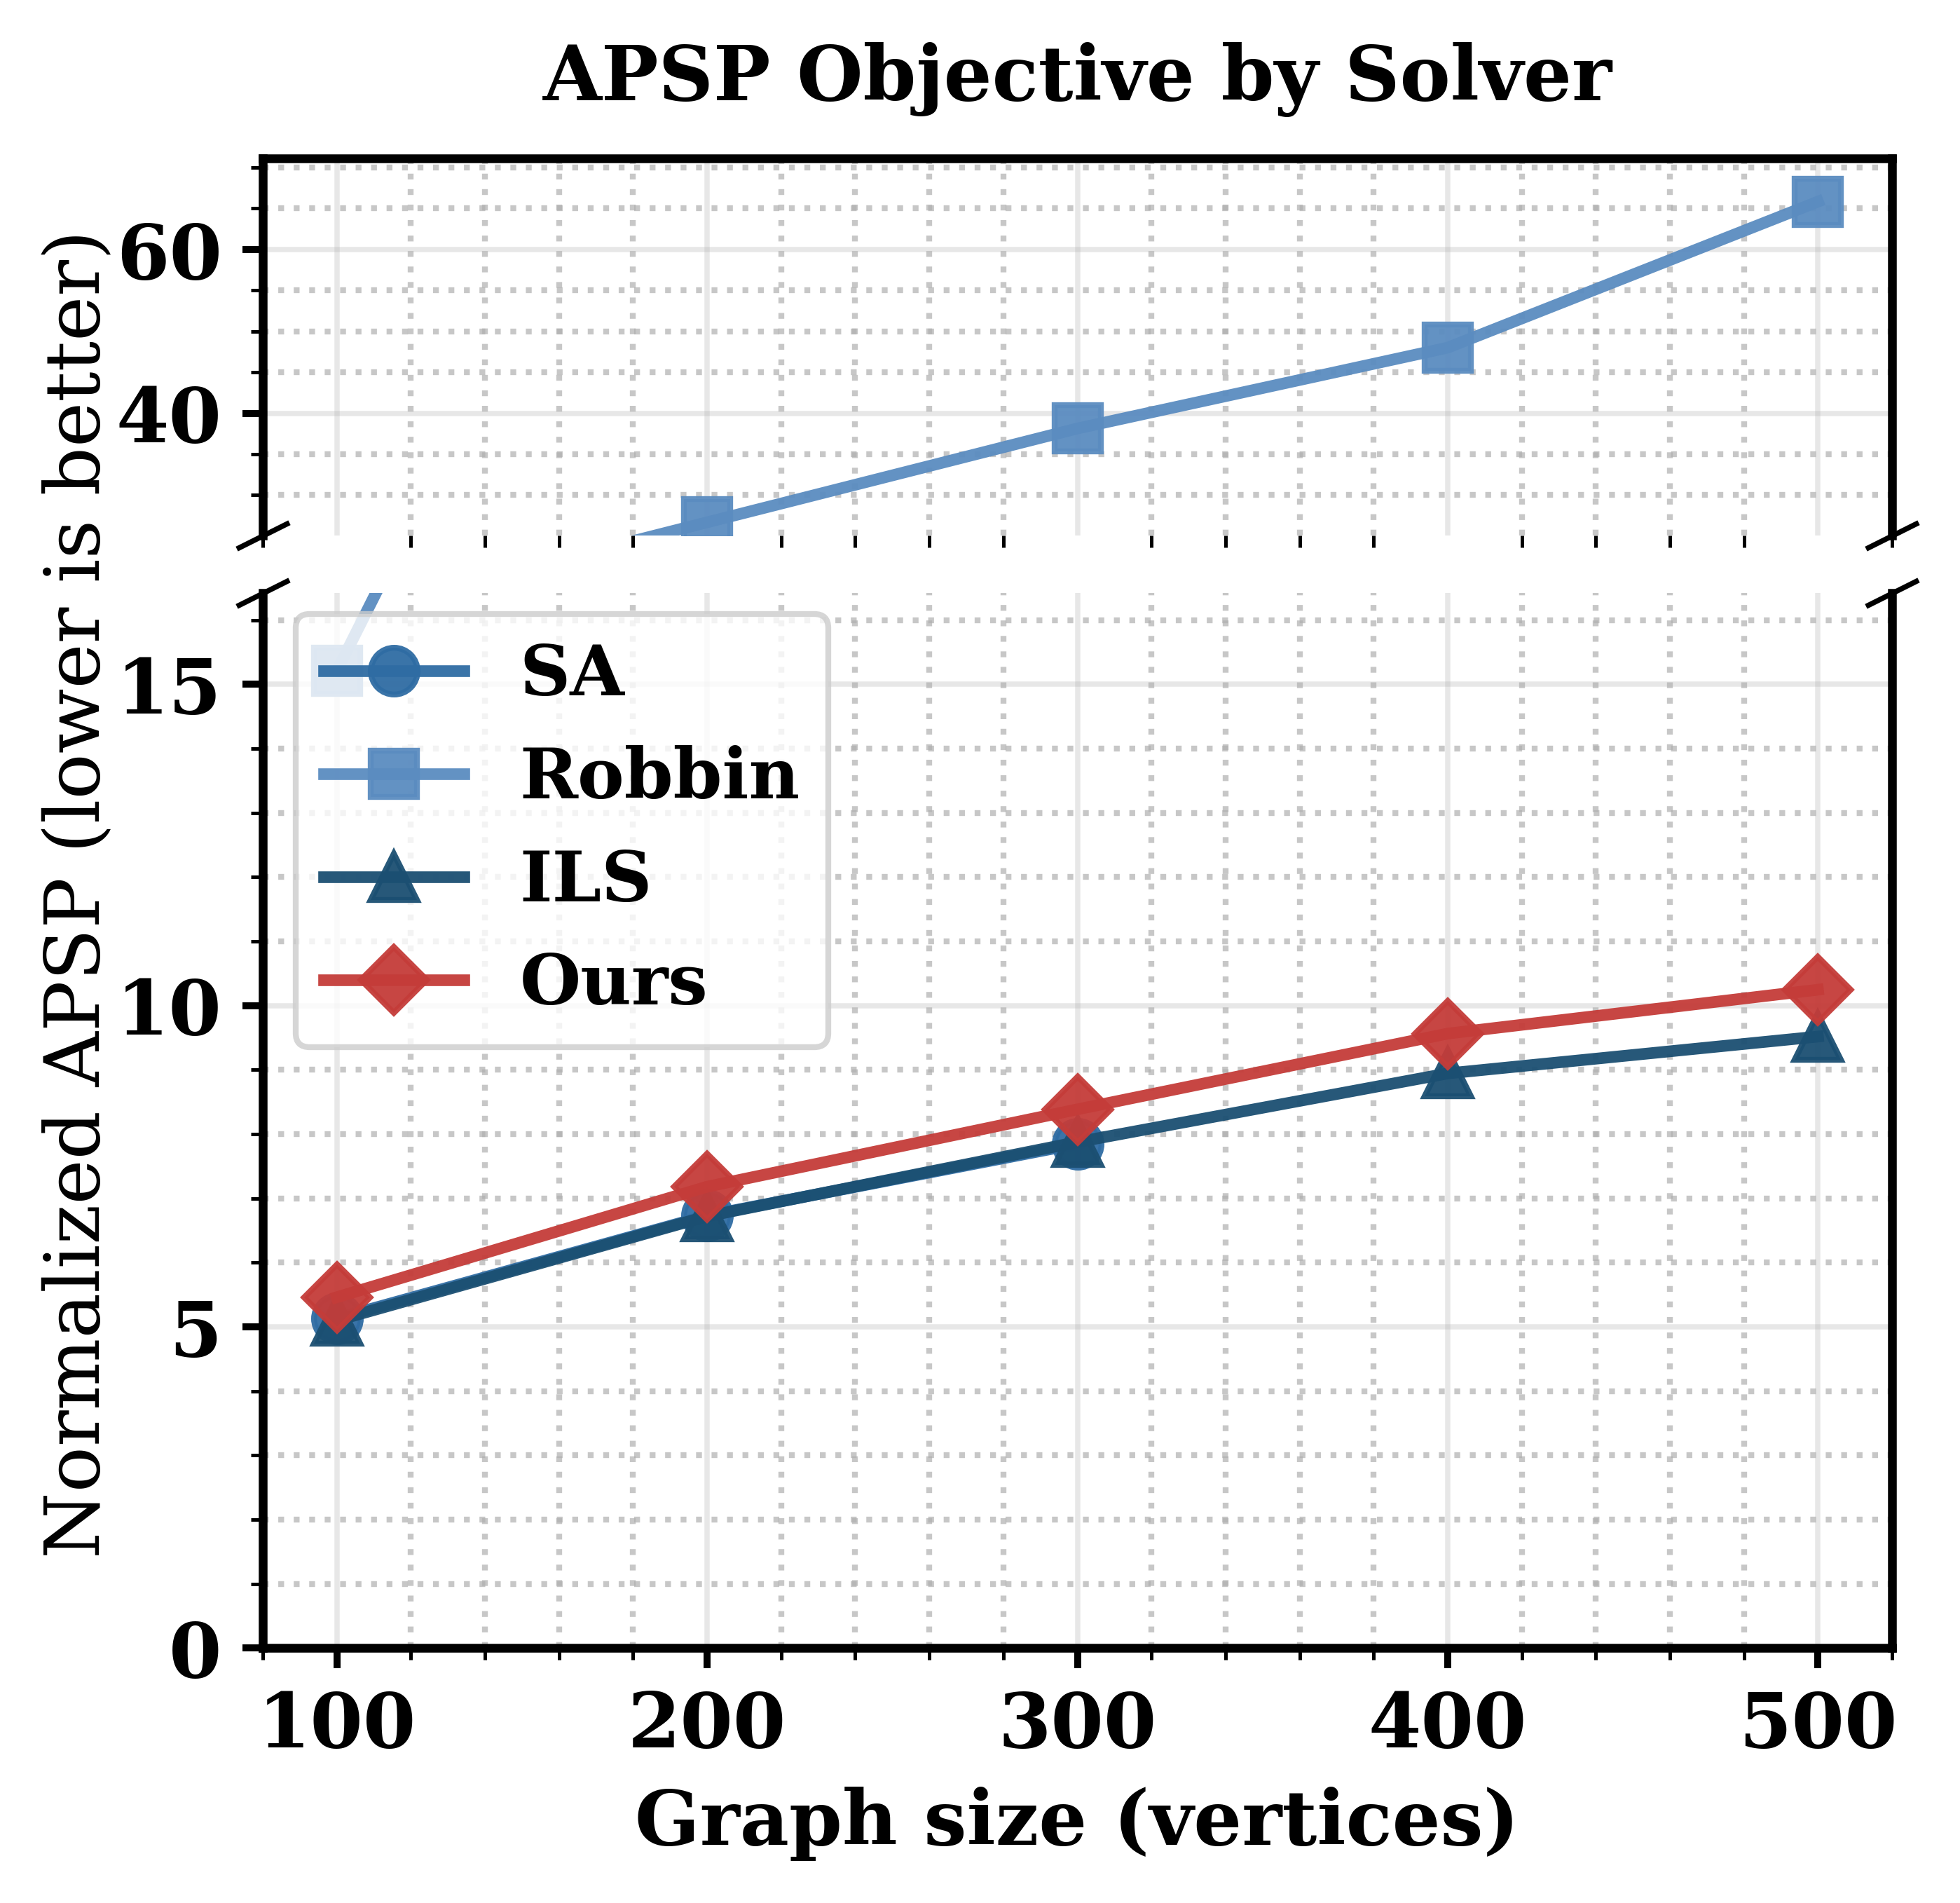
\includegraphics[width=\linewidth]{../ko/fig/apsp_reduction.png}
\caption{Mean directed shortest-path distance \(D_{\mathrm{avg}}\) after orientation (lower is better; averaged over three instances, except \(|V|=200\) for the proposed method, which averages two). SA denotes Raw SA and Ours denotes the proposed method. Raw SA is omitted for \(|V|\geq400\), where it obtains no strongly connected orientation.}
\label{fig:apsp}
\end{figure}

Because \(D_{\mathrm{avg}}\) is normalized only by the number of ordered pairs, it grows with the graph. To enable cross-size comparison, Figure~\ref{fig:stretch} replots the same results as the ratio by which orientation stretches the pre-orientation distances. The undirected mean distance \(\bar{D}_{\mathrm{avg}}\) was obtained by regenerating each instance from the same seed, and equals 4.271, 5.671, 6.633, 7.643 and 8.097 at \(|V|=100,200,300,400,500\). The ratio of the proposed method is 1.28, 1.27, 1.26, 1.25 and 1.27, that is, flat in the graph size; ILS stays within 1.17--1.19, whereas Robbins grows from 3.56 to 8.13. The apparent degradation with size in Figure~\ref{fig:apsp} is therefore an effect of the graph growing rather than of the orientation quality deteriorating, and the gap between the proposed method and ILS does not widen with size.

The values in Figure~\ref{fig:stretch} are, however, the ratio of the means \(D_{\mathrm{avg}}/\bar{D}_{\mathrm{avg}}\) and not the \(F_{\mathrm{dist}}\) of \eqref{eq:stretch}. Since \(F_{\mathrm{dist}}\) is the mean of the per-pair ratios, computing it requires the orientation each method actually produced, and those orientations were not retained in the experimental records, so they could not be recovered after the fact. The two quantities do not coincide: comparing them directly on the same instances under a Robbins-style orientation, the ratio of the means falls 4--10\% below \(F_{\mathrm{dist}}\), because pairs at short undirected distance are stretched the most and the ratio of the means underweights them. The values in Figure~\ref{fig:stretch} should accordingly be read as a lower bound on \(F_{\mathrm{dist}}\).

\begin{figure}[t]
\centering
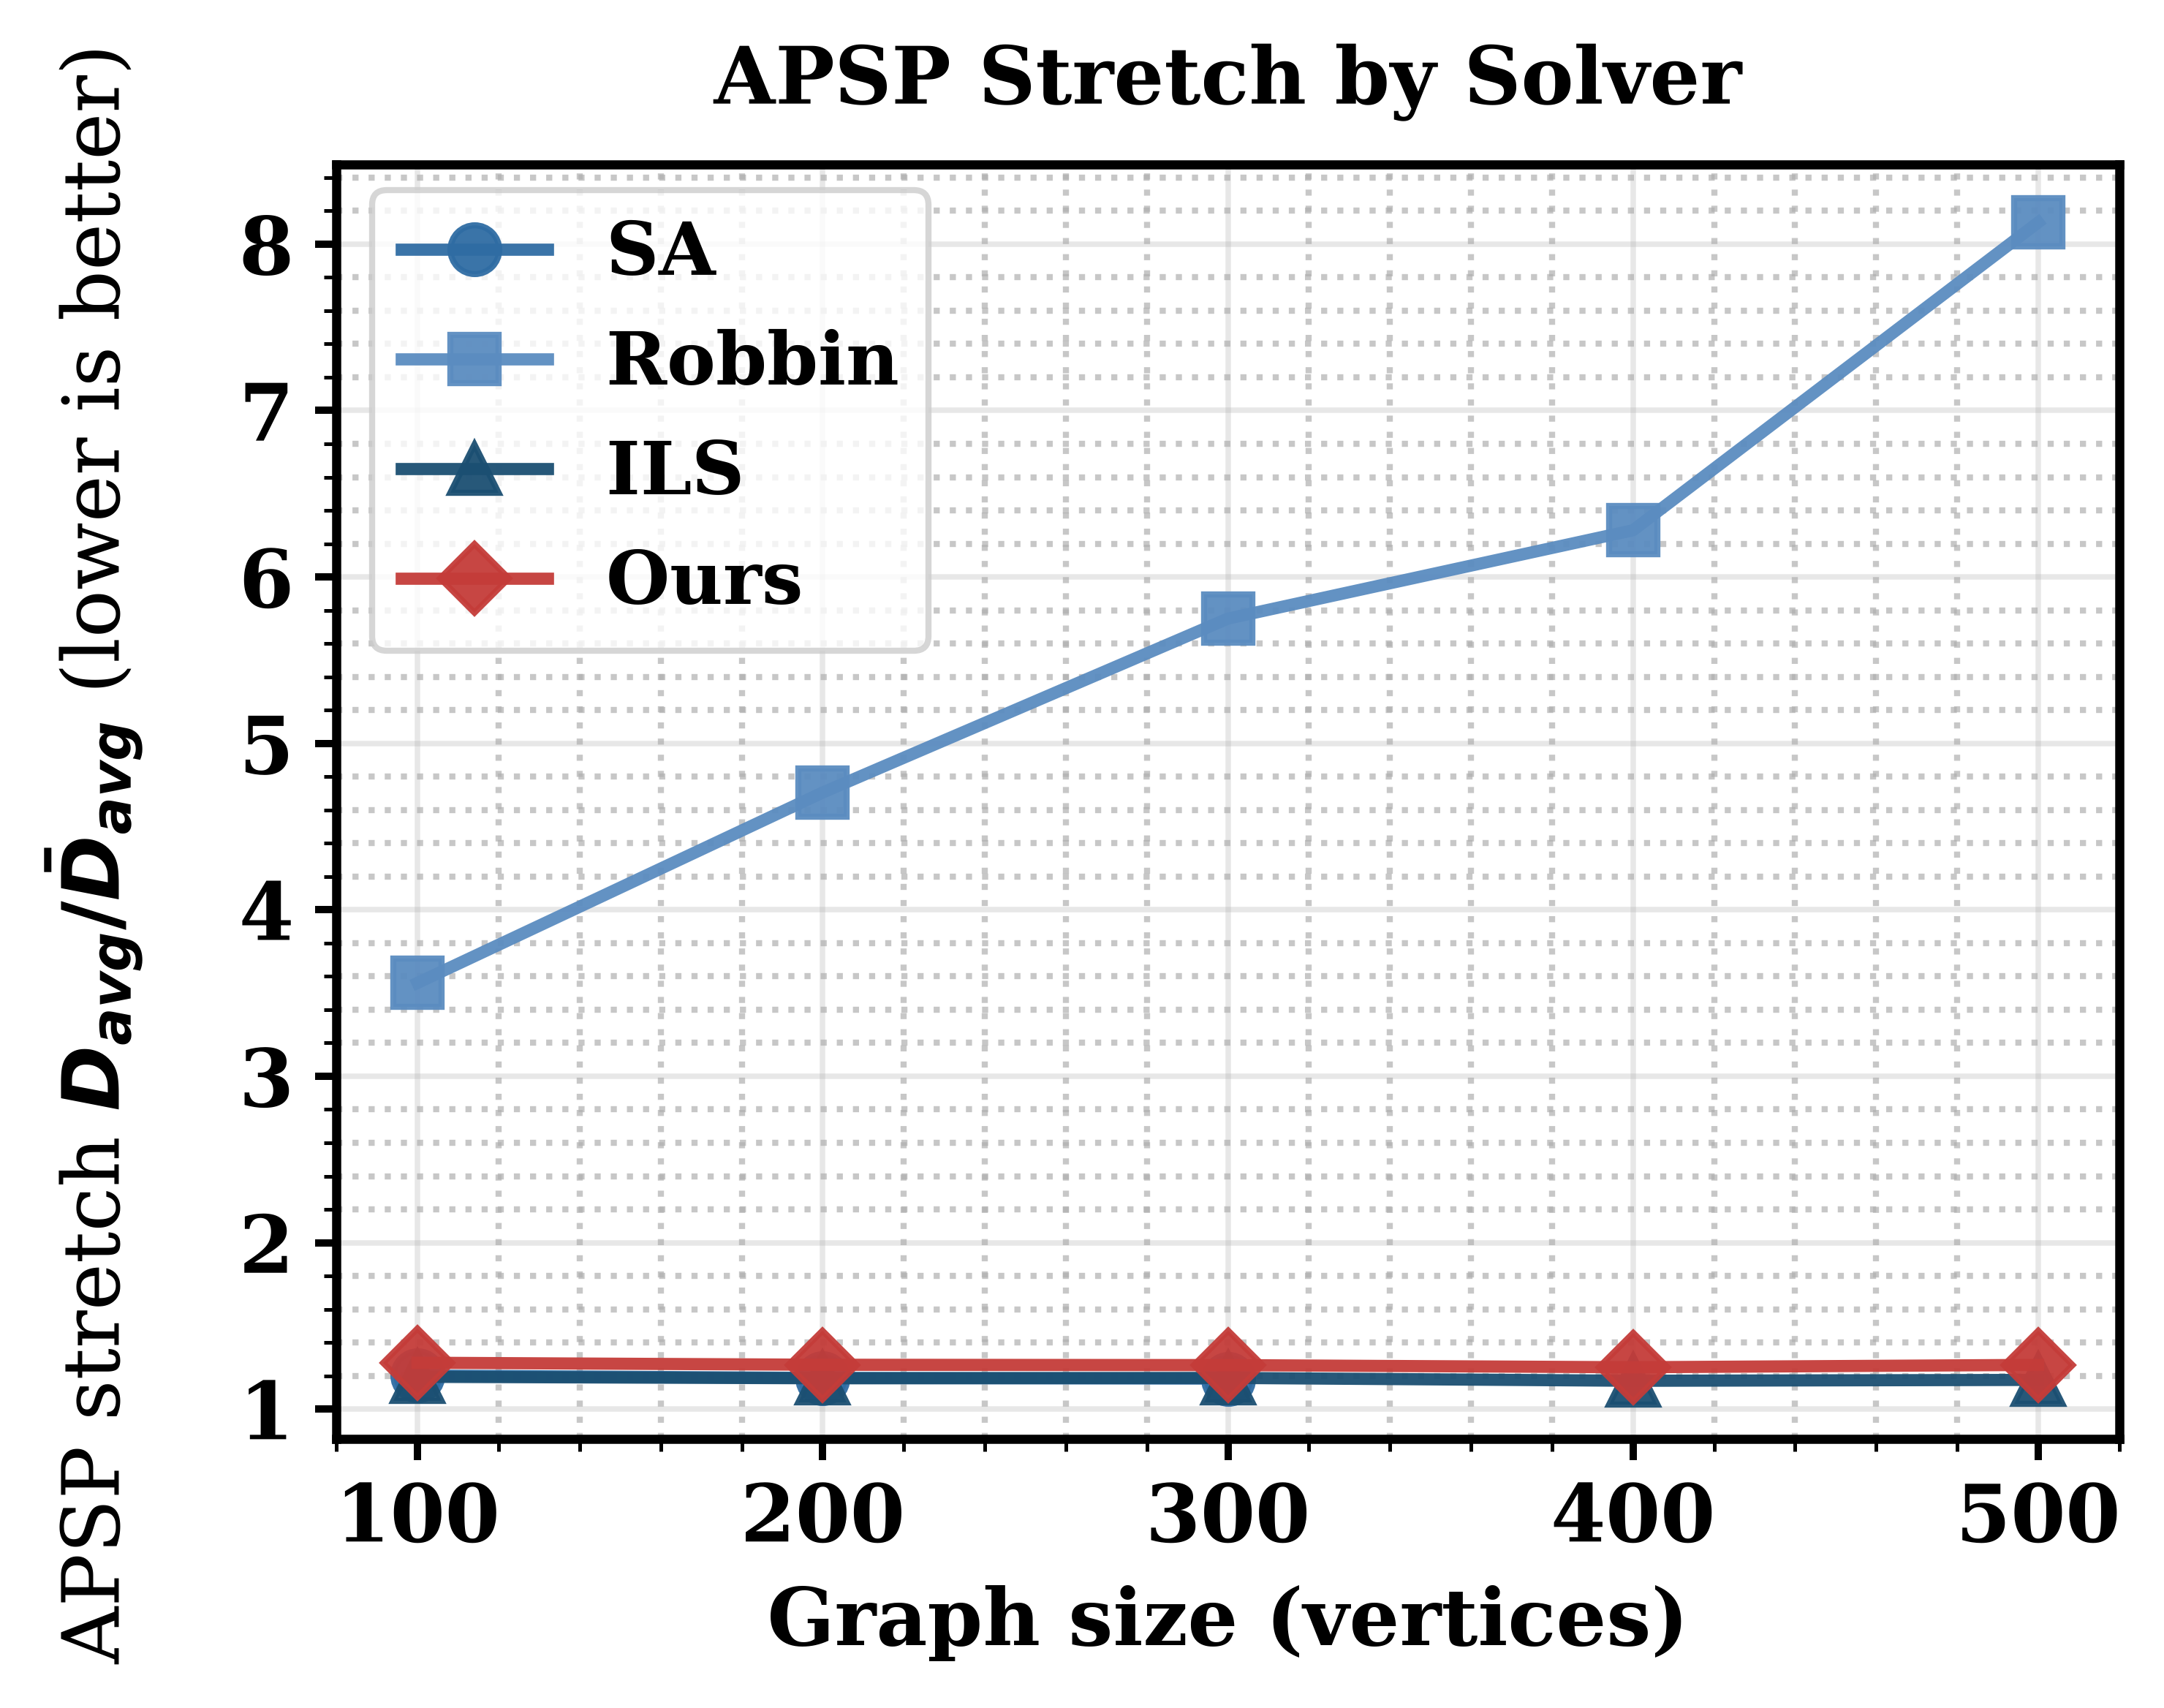
\includegraphics[width=\linewidth]{../ko/fig/apsp_stretch.png}
\caption{Distance stretch induced by orientation, \(D_{\mathrm{avg}}/\bar{D}_{\mathrm{avg}}\) (lower is better; a value of one means the orientation preserves the original distances exactly). The experiment of Figure~\ref{fig:apsp} is divided by the undirected reference distance, which puts networks of different sizes on a common axis. The \(F_{\mathrm{dist}}\) of \eqref{eq:stretch} is the mean of the per-pair ratios and therefore differs from this quantity, which falls 4--10\% below it.}
\label{fig:stretch}
\end{figure}

\subsection{Runtime}

The mean per-instance runtime splits into two parts. QUBO solving takes 16.9 seconds at \(|V|=500\), against 429 seconds for solving the unpartitioned whole-graph QUBO by classical simulated annealing. The embedding search, by contrast, takes 4{,}243 seconds and dominates the solving time, because a search is performed for every subgraph; the 1{,}064 seconds of the unpartitioned case is mostly the cost of a single search that ends in failure. Robbins, a classical method, is the fastest at 3.5 seconds, but its solution quality is far worse, as Figure~\ref{fig:apsp} shows.

In short, the dominant cost in the current implementation is not QUBO solving but the embedding search.

\subsection{Validity of the \(n\)-Hop Surrogate}

A separate experiment verified that the surrogate objective of Section~\ref{subsec:model_hop} is in fact correlated with distance. On a Delaunay graph with 50 vertices and 137 edges, we drew 500 random strongly connected orientations and measured, for each, both the sum of directed shortest-path distances and the number of \(n\)-hop reachable pairs. Here the number of \(n\)-hop reachable pairs is the number of ordered pairs joined by a simple path of exactly \(n\) edges; it is not \(P_n\) itself, which is a weighted walk count, but it is a surrogate quantity that counts the same structure under unit weights.

\begin{figure*}[t]
\centering
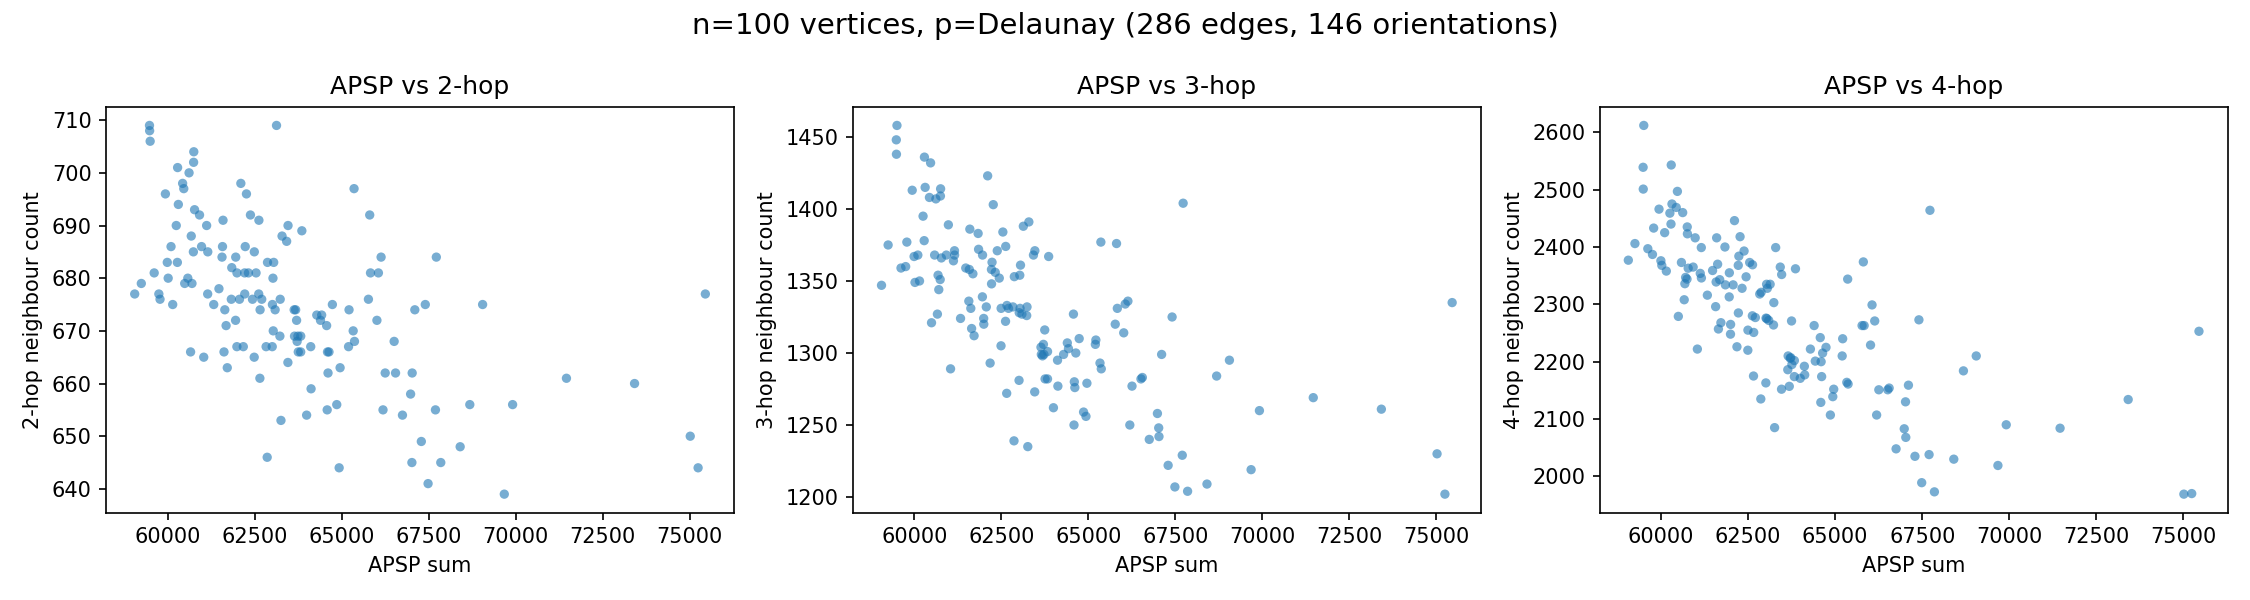
\includegraphics[width=\textwidth]{../ko/fig/nhop_apsp.png}
\caption{Relationship between the sum of directed shortest-path distances and the number of \(n\)-hop reachable pairs (50 vertices, 137 edges, 500 orientations). From left to right, \(n=2,3,4\).}
\label{fig:nhop}
\end{figure*}

All three hop lengths show a clear negative correlation in Figure~\ref{fig:nhop}. That is, orientations with more \(n\)-hop reachable pairs have a smaller distance sum, which supports the use of maximizing \(P_n\) as a surrogate for minimizing distance on this instance. Judged by correlation strength alone, however, \(n=4\) is better than \(n=2\). The grounds for restricting the hop length to \(\{2,3\}\) are therefore not the relative strength of the correlations but the degree condition of Proposition~\ref{prop:deg}. Including \(n=4\) would make the objective quartic, requiring degree reduction and auxiliary variables, and would further increase the coupling density that already reaches its limit in Section~\ref{subsec:result_embed}. The same trend was confirmed on a 100-vertex graph at the experimental scale (146 orientations). Because this is a single-graph experiment, we do not report correlation coefficients.

\subsection{Hop-Length Ablation and Coupling Measurements} \label{subsec:result_ablation}

To separate the cost and the benefit of the \(P_3\) term, we compared two configurations on the same 15 instances, \(\lambda_3=1\) (hop23) and \(\lambda_3=0\) (hop2), both at the effective \(\lambda_2=5\) of Remark~\ref{rmk:flow}, using classical simulated annealing (20 samples). Figure~\ref{fig:ablation} summarizes the results.

\begin{figure*}[t]
\centering
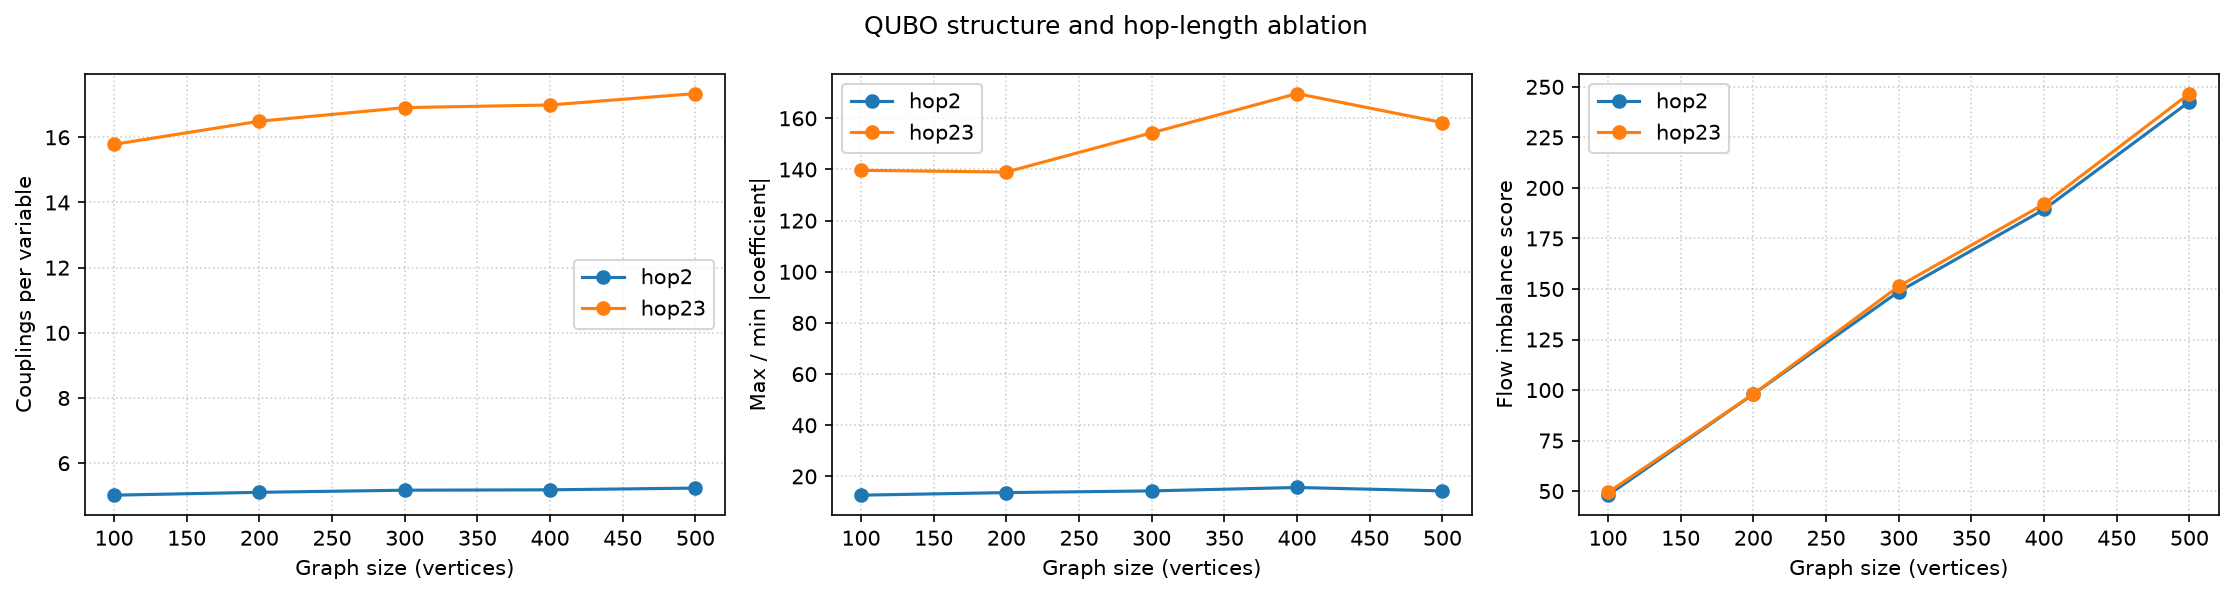
\includegraphics[width=\textwidth]{../ko/fig/qubo_structure.png}
\caption{Hop-length ablation. From left to right: couplings per variable, ratio of maximum to minimum coefficient, and directed distance sum. hop23 uses \(\lambda_3=1\) and hop2 uses \(\lambda_3=0\).}
\label{fig:ablation}
\end{figure*}

The cost side is unambiguous. Including \(P_3\) raises the number of couplings per variable from 5.0--5.2 to 15.8--17.3, a factor of 3.2; widens the ratio of maximum to minimum coefficient from 13--16 to 140--170, an order of magnitude; and increases the solving time by a factor of 3.2 at \(|V|=500\), from 97 to 311 seconds. These are the coupling measurements anticipated in Section~\ref{subsec:method_partition}: at \(|V|=500\) the coupling count is 25{,}678, roughly 17 times the number of edges.

No benefit was observed. Across the 15 instances the distance sum was lower for hop23 in 8 cases and for hop2 in 7, with a maximum difference of 1.1\%, which lies within the instance-to-instance spread, and strong connectivity was achieved in all 15 trials for both configurations. In other words, on this family of instances \(P_3\) tripled the coupling density that creates the embedding limit of Section~\ref{subsec:result_embed} without improving solution quality. Whether the \(\lambda_3=0\) configuration can embed larger graphs without partitioning is left as future work.

\section{Conclusion} \label{sec:conclusion}

This study formulated the strongly connected orientation problem for pedestrian networks as a QUBO free of auxiliary variables and proposed a framework that solves it on a D-Wave quantum annealer. The property that walks pair with their reversals so that the highest-degree terms cancel (Proposition~\ref{prop:deg}) keeps the \(n\)-hop objective quadratic, and the strong-connectivity constraint is handled not by a penalty term but by series contraction and face partitioning with boundary pre-orientation (Proposition~\ref{prop:sc}), which eliminates the tuning of penalty weights.

The central experimental finding is a trade-off between time and quality. In solution quality, ILS, which minimizes the evaluation metric directly, attains the lowest \(D_{\mathrm{avg}}\) at every size, but requires 44{,}862 seconds per instance at \(|V|=500\). At the same size the proposed method takes 4{,}260 seconds in total, roughly one tenth of ILS, while achieving a \(D_{\mathrm{avg}}\) more than six times lower than that of Robbins together with strong connectivity in every completed trial. Since \(D_{\mathrm{avg}}\) itself grows with the graph, measured by the stretch relative to the pre-orientation distances the proposed method stays flat at 1.25--1.28 across all sizes, and its gap to ILS (1.17--1.19) does not widen with size (Figure~\ref{fig:stretch}). The proposed method thus offers not the best quality but a practical compromise between quality and computation time while maintaining strong connectivity.

Three limitations remain. First, the solution quality falls short of ILS, a structural gap that arises because the QUBO minimizes the surrogate objective \(H\). Second, most of the total time (4{,}243 of 4{,}260 seconds) is spent not on QUBO solving but on the minor-embedding search, so the current bottleneck is classical preprocessing rather than quantum hardware. Third, the \(P_3\) term multiplies the coupling density by 3.2, creating the embedding limit, without any observed improvement in solution quality.

As future work we plan to narrow the scope of pre-orientation. The current construction pre-orients the entire outer cycle of each face in a single direction, so every boundary edge is removed from the decision variables and the freedom of the solution is restricted. Pre-orientation is, however, genuinely needed only on the edges shared by two faces: if these are left free, adjacent subproblems may return conflicting directions for the same edge. Fixing only these shared edges as a set of fixed edges and leaving the remaining boundary edges as decision variables would open a larger solution space under the same hardware constraints. We further plan to explore searching for the best configuration by iteratively varying the choice of directions on the fixed edge set.

\bibliographystyle{plain}
\bibliography{../../AQC/Fig_MaiDinhCong/ref}

\end{document}
